\documentclass[a4paper,11pt]{article}

% Kodovani (cestiny) v dokumentu: utf-8
%\usepackage[cp1250]{inputenc}	% Omezena stredoevropska kodova stranka, pouze MSW.
\usepackage[utf8]{inputenc}	% Doporucujeme pouzivat UTF-8 (unicode).

\usepackage[margin=2cm]{geometry}
\newtoks\jmenopraktika \newtoks\jmeno \newtoks\datum
\newtoks\obor \newtoks\skupina \newtoks\rocnik \newtoks\semestr
\newtoks\cisloulohy \newtoks\jmenoulohy
\newtoks\tlak \newtoks\teplota \newtoks\vlhkost

\jmenopraktika={Fyzikální praktikum 1}
\jmeno={Lukáš Lejdar}
\datum={24. září 2024}
\obor={F}
\skupina={Út 16:00}

\cisloulohy={5}
\jmenoulohy={Magnetické pole}

\tlak={101{,}35}
\teplota={21,1}
\vlhkost={47,7}


%%%%%%%%%%% Uzitecne balicky:
\usepackage[czech]{babel}
\addto\captionsczech{\renewcommand{\figurename}{Obrázek}}

\usepackage{graphicx}
\usepackage{amsmath}
\usepackage{xspace}
\usepackage{url}
\usepackage{indentfirst}
\usepackage{wrapfig}
\usepackage{xcolor}
\usepackage{subfig}
\usepackage{subcaption}
\usepackage{newfloat}

\DeclareFloatingEnvironment[fileext=lof]{graph}
\captionsetup[graph]{labelformat=simple, labelsep=colon, name=Graf}

%%%%%% Zamezeni parchantu:
\widowpenalty 10000 \clubpenalty 10000 \displaywidowpenalty 10000
%%%%%% Parametry pro moznost vsazeni vetsiho poctu obrazku na stranku
\setcounter{topnumber}{3}	  % max. pocet floatu nahore (specifikace t)
\setcounter{bottomnumber}{3}	  % max. pocet floatu dole (specifikace b)
\setcounter{totalnumber}{6}	  % max. pocet floatu na strance celkem
\renewcommand\topfraction{0.9}	  % max podil stranky pro floaty nahore
\renewcommand\bottomfraction{0.9} % max podil stranky pro floaty dole
\renewcommand\textfraction{0.1}	  % min podil stranky, ktery musi obsahovat text
\intextsep=8mm \textfloatsep=8mm  %\intextsep pro ulozeni [h] floatu a \textfloatsep pro [b] or [t]

% Tecky za cisly sekci:
\renewcommand{\thesection}{\arabic{section}.}
\renewcommand{\thesubsection}{\thesection\arabic{subsection}.}
% Jednopismenna mezera mezi cislem a nazvem kapitoly:
\makeatletter \def\@seccntformat#1{\csname the#1\endcsname\hspace{1ex}} \makeatother
%
\newcommand{\vsn}[4]{\ensuremath{#1 =} #2(#3)\,#4}
\newcommand{\vrn}[6]{\ensuremath{#1 =} (#2 $\pm$ #3)\,#4 ($p=$ #5\,\%, $\nu=$ #6)}


%%%%%%%%%%%%%%%%%%%%%%%%%%%%%%%%%%%%%%%%%%%%%%%%%%%%%%%%%%%%%%%%%%%%%%%%%%%%%%%
% Zacatek dokumentu
%%%%%%%%%%%%%%%%%%%%%%%%%%%%%%%%%%%%%%%%%%%%%%%%%%%%%%%%%%%%%%%%%%%%%%%%%%%%%%%

\begin{document}

\thispagestyle{empty}

{
\begin{center}
\sf 
{\Large Ústav fyziky a technologií plazmatu Přírodovědecké fakulty Masarykovy univerzity} \\
\bigskip
{\huge \bfseries FYZIKÁLNÍ PRAKTIKUM} \\
\bigskip
{\Large \the\jmenopraktika}
\end{center}

\bigskip

\sf
\noindent
\setlength{\arrayrulewidth}{1pt}
\begin{tabular*}{\textwidth}{@{\extracolsep{\fill}} l l}
\large {\bfseries Zpracoval:}  \the\jmeno & \large  {\bfseries Naměřeno:} \the\datum\\[2mm]
\large  {\bfseries Obor:} \the\obor  \hspace{40mm}  {\bfseries Skupina:} \the\skupina %
&\large {\bfseries Testováno:}\\
\\
\hline
\end{tabular*}
}

\bigskip

{
\sf
\noindent \begin{tabular}{p{4cm} p{0.6\textwidth}}
\Large  Úloha č. {\bfseries \the\cisloulohy:} \par
\smallskip
$T=\the\teplota$~$^\circ$C \par
$p=\the\tlak$~kPa \par
$\varphi=\the\vlhkost$~\%
&\Large \bfseries \the\jmenoulohy  \\[2mm]
\end{tabular}
}

\vskip1cm

\section{Úvod}

Cílem je změřit horizontální složku magnetického pole na Zemi pomocí Gaussova magnetometru a proměřit magnetickou odezvu feromagnetického materiálu.
 
\section{Postup měření}

\subsection{Geomagnetické pole}

Máme střelkový kompas a tyčový magnet v konfiguraci podle Gaussových poloh 1 a 2 jako na obrázku 1. Pokud délka magnetu \( l \) je výrazně menší než vzdálenost od kompasu \( r \) a magnet považujeme za nekonečně tenký, lze odvodit aproximativní vztah

\begin{equation}
    H_z = \frac{7M}{4 \pi \mu_0 r^3} \frac{1}{ \left( \frac{3}{2}\tan \varphi_1 + 4 \tan \varphi_2  \right) },
\end{equation}

\noindent
kde \( M = \mu l \) je celkový magnetický moment, který určíme z periody kmitů v magnetickém poli Země. Je-li osa magnetu stočena vůči magnetickému poli Země o úhel \( \varphi \), pak na něj působí magnetický moment velikosti
$ M H_z \sin \varphi \approx M H_z \varphi $
a pokud direkční moment závěsu $ D \varphi \approx 0 $, platí pohybová rovnice
\begin{equation}
 J \ddot \varphi + M H_z \varphi = 0 ,
\end{equation}

\noindent
kde 

\begin{equation}
J = \frac{m}{4} \left(R^2 + \frac{l^2}{3} \right)
\end{equation}

\noindent
je moment setrvačnosti válce. Celý magnet potom na závěsu kmitá s periodou

\begin{equation}
T^2 = \frac{4 \pi^2 J}{M H_z}
\end{equation}

\noindent
odkud lze dosadit do vztahu 1.

\begin{equation}
    H_z = \frac{1}{T} \sqrt{ \frac{7 \pi J }{\mu_0 r^3} \frac{1}{ \left( \frac{3}{2}\tan \varphi_1 + 4 \tan \varphi_2  \right) } }
\end{equation}


\begin{figure}[htpb]
    \centering
    \includegraphics[width=0.6\textwidth]{usporadani.png}
    \caption{Schéma experimentálního uspořádání. Permanentní magnet je vždy
orientován kolmo ke směru magnetického pole Země podél osy x a úhly \( \varphi_1 \) a \( \varphi_2 \) označují výchylky střelky kompasu od severo-jižního směru. }
\end{figure}

\subsection{Magnetické odezva feromagnetického materiálu}

Hledáme způsob, jak zjistit parametrickou závislost magnetické indukce $ y = B(t) $ na magnetické intenzitě $ x = H(t) $ v některém materiálu. Pro tento účel slouží obvod na obrázku~2, kde měření probíhá na tenkém toroidním magnetickém jádře se dvěma vinutími buzeném střídavým napětím $ U = U_0 \cos (\omega t) $. Pro obvod primárního vynutí můžeme získat první závislost z Ampérova zákona jako


\begin{equation}
H(t) = \frac{N_1 I_1}{2 \pi r} = \frac{N_1 }{2 \pi r R_1} U_1(t)
\end{equation}

Pro zjednodušení budu předpokládat konstantní intenzitu magnetického pole i magnetickou indukčnost, aby platilo $ \Phi = S N B  $ a $ \textbf{B}(t) = \mu_0 ( \textbf{H}(t) + \textbf{M}(t) ) $, kde do vztahu (6) dosadím průměr poloměrů $ r_{\rm max} $ a $ r_{\rm min} $. Pro obvod sekundárního vinutí platí


\begin{align}
    \frac{d\phi}{dt} + R_2C\dot{U}_C + U_C = 0.
\end{align}

Je-li časová konstanta integračniho obvodu $ R_2C \gg T = \frac{2\pi}{\omega} $, pak lze okamžitý náboj na kondenzátoru~ohraničit jako $| C U_C | = | Q_C | \le  T \dot{U}_{C}^{Amp} \ll R_2C \dot{U}_{C}^{Amp}$ odkud plyne, že po většinu času periody platí $ U_C \ll R_2C \dot{U}_C $. Jinými slovy, kondenzátor se nikdy nestihne nabít a člen $ U_C $ v rovnici (6) můžeme zanedbat. Když navíc dosadím $ \frac{d \Phi}{dt} = N_2 S_2 \frac{dB}{dt} $ dostávám druhou závislost


\begin{equation}
B(t) \approx - \frac{R_2C}{N_2 S_2} U_C(t)
\end{equation}


\begin{table}[htpb]
    \vspace{-10pt}
    \hfill
    \begin{minipage}[b]{.50\textwidth}
    \centering
    \includegraphics[width=1\textwidth]{obvod.png}
    \captionsetup{type=figure}
    \caption{Schéma obvodu pro měření magnetického pole ve feromagnetu}
    \end{minipage}
    \hfill
    \vspace{-40pt}
    \begin{minipage}[b]{.23\textwidth}
        \centering
        \includegraphics[width=1\textwidth]{toroid.png}
        \captionsetup{type=figure}
        \caption{Schéma řezu toroidní cívkou}
    \end{minipage}
    \hfill
    \hfill
\end{table}

\newpage


\section{Výsledky měření}

\subsection{Geomagnetické pole}

Použil jsem válcový magnet o hmotnosti $ m = 306.3 \pm 0.2\ g $, délce $ l = 123.3 \pm 0.4\ mm $ a průměru $ d = 21.2 \pm 0.1\ mm $, který při vodorovném závěsu kmitá s periodou $ T = 9.62 \pm 0.04\ s $. Výchylky střelky kompasu $\varphi$ způsobené tímto magnetem v Gaussových poloháh 1 a 2 jsou uvedené v tabulce 1.

\begin{table}[htpb]
  \centering
   \begin{tabular}{ | c | c | c | c | c |  c |}
       \hline
       r $\pm$ 0.5 (mm) & \( \varphi_1^+ \) $\pm$ 1 & \( \varphi_1^- \) $\pm$ 1& \( \varphi_2^+ \) $\pm$ 1& \( \varphi_2^- \) $\pm$ 1 \\
       \hline
       -300  & 73 & -75 & -50 & 52 \\
       -400 & 52 & -50 & -33 & 35 \\
       -500 & 37 & -37 & -19 & 22 \\
       300  & 72 & -71 & -50 & 53 \\ 
       400  & 51 & -51 & -34 & 33 \\
       500  & 37 & -36 & -19 & 19 \\    
       \hline
   \end{tabular}
   \caption{Měření výchylky střelky kompasu od severo-jižního směru pro obě natočení magnetu v obou Gaussových poloháh.}
\end{table}

Pro každou dvojici úhlů $ \varphi $ jsem podle vztahu (6) spočítal horizontální komponentu magnetického pole země a výsledné hodnoty zprůměroval pro konečné

\begin{equation}
H_z = 16.2  \pm 0.3 \ Am^{-1}
\end{equation}

\subsection{Magnetické odezva feromagnetického materiálu}

Sestavil jsem obvod podle obrázku 2 s parametry $ R_1 = 83\ \Omega $, $ R_2 = 120\ k\Omega $, $ C = 1\ \mu F $. Počty závitů na okruzích transformátoru byly $ N_1 = 260$ a $ N_2 = 900 $ s toroidním feromagnetickým jádrem o rozměrech $ r_2 = 28.7 \pm 0.3 \ mm $, $ r_1 = 19.5 \pm 0.3 \ mm $ a výškou $ h = 7.3 \pm 0.2 \ mm $. Měřil jsem závislost $ U_C(t) $ a $ U_1(t) $ a podle vztahů (8) a (6) vykreslil závislost $ B $ na $ H $ do grafu 1.

Získaná saturační magnetizace je $B_s = 0.169$ $ T $ pro intenzitu $H_s = 86.6$ $ Am^{-1} $, koercitivní síla $ H_C = 29.1\ Am^{-1} $ a remanentní magnetizace $ B_R = 0.126 $ $ T $.


\begin{figure}[htpb]
    \centering
    % GNUPLOT: LaTeX picture with Postscript
\begingroup
  \makeatletter
  \providecommand\color[2][]{%
    \GenericError{(gnuplot) \space\space\space\@spaces}{%
      Package color not loaded in conjunction with
      terminal option `colourtext'%
    }{See the gnuplot documentation for explanation.%
    }{Either use 'blacktext' in gnuplot or load the package
      color.sty in LaTeX.}%
    \renewcommand\color[2][]{}%
  }%
  \providecommand\includegraphics[2][]{%
    \GenericError{(gnuplot) \space\space\space\@spaces}{%
      Package graphicx or graphics not loaded%
    }{See the gnuplot documentation for explanation.%
    }{The gnuplot epslatex terminal needs graphicx.sty or graphics.sty.}%
    \renewcommand\includegraphics[2][]{}%
  }%
  \providecommand\rotatebox[2]{#2}%
  \@ifundefined{ifGPcolor}{%
    \newif\ifGPcolor
    \GPcolorfalse
  }{}%
  \@ifundefined{ifGPblacktext}{%
    \newif\ifGPblacktext
    \GPblacktexttrue
  }{}%
  % define a \g@addto@macro without @ in the name:
  \let\gplgaddtomacro\g@addto@macro
  % define empty templates for all commands taking text:
  \gdef\gplbacktext{}%
  \gdef\gplfronttext{}%
  \makeatother
  \ifGPblacktext
    % no textcolor at all
    \def\colorrgb#1{}%
    \def\colorgray#1{}%
  \else
    % gray or color?
    \ifGPcolor
      \def\colorrgb#1{\color[rgb]{#1}}%
      \def\colorgray#1{\color[gray]{#1}}%
      \expandafter\def\csname LTw\endcsname{\color{white}}%
      \expandafter\def\csname LTb\endcsname{\color{black}}%
      \expandafter\def\csname LTa\endcsname{\color{black}}%
      \expandafter\def\csname LT0\endcsname{\color[rgb]{1,0,0}}%
      \expandafter\def\csname LT1\endcsname{\color[rgb]{0,1,0}}%
      \expandafter\def\csname LT2\endcsname{\color[rgb]{0,0,1}}%
      \expandafter\def\csname LT3\endcsname{\color[rgb]{1,0,1}}%
      \expandafter\def\csname LT4\endcsname{\color[rgb]{0,1,1}}%
      \expandafter\def\csname LT5\endcsname{\color[rgb]{1,1,0}}%
      \expandafter\def\csname LT6\endcsname{\color[rgb]{0,0,0}}%
      \expandafter\def\csname LT7\endcsname{\color[rgb]{1,0.3,0}}%
      \expandafter\def\csname LT8\endcsname{\color[rgb]{0.5,0.5,0.5}}%
    \else
      % gray
      \def\colorrgb#1{\color{black}}%
      \def\colorgray#1{\color[gray]{#1}}%
      \expandafter\def\csname LTw\endcsname{\color{white}}%
      \expandafter\def\csname LTb\endcsname{\color{black}}%
      \expandafter\def\csname LTa\endcsname{\color{black}}%
      \expandafter\def\csname LT0\endcsname{\color{black}}%
      \expandafter\def\csname LT1\endcsname{\color{black}}%
      \expandafter\def\csname LT2\endcsname{\color{black}}%
      \expandafter\def\csname LT3\endcsname{\color{black}}%
      \expandafter\def\csname LT4\endcsname{\color{black}}%
      \expandafter\def\csname LT5\endcsname{\color{black}}%
      \expandafter\def\csname LT6\endcsname{\color{black}}%
      \expandafter\def\csname LT7\endcsname{\color{black}}%
      \expandafter\def\csname LT8\endcsname{\color{black}}%
    \fi
  \fi
    \setlength{\unitlength}{0.0500bp}%
    \ifx\gptboxheight\undefined%
      \newlength{\gptboxheight}%
      \newlength{\gptboxwidth}%
      \newsavebox{\gptboxtext}%
    \fi%
    \setlength{\fboxrule}{0.5pt}%
    \setlength{\fboxsep}{1pt}%
    \definecolor{tbcol}{rgb}{1,1,1}%
\begin{picture}(5760.00,3600.00)%
    \gplgaddtomacro\gplbacktext{%
      \csname LTb\endcsname%%
      \put(-132,108){\makebox(0,0)[r]{\strut{}$-0.2$}}%
      \put(-132,544){\makebox(0,0)[r]{\strut{}$-0.15$}}%
      \put(-132,981){\makebox(0,0)[r]{\strut{}$-0.1$}}%
      \put(-132,1417){\makebox(0,0)[r]{\strut{}$-0.05$}}%
      \put(-132,1854){\makebox(0,0)[r]{\strut{}$0$}}%
      \put(-132,2290){\makebox(0,0)[r]{\strut{}$0.05$}}%
      \put(-132,2726){\makebox(0,0)[r]{\strut{}$0.1$}}%
      \put(-132,3163){\makebox(0,0)[r]{\strut{}$0.15$}}%
      \put(-132,3599){\makebox(0,0)[r]{\strut{}$0.2$}}%
      \put(0,-112){\makebox(0,0){\strut{}$-100$}}%
      \put(576,-112){\makebox(0,0){\strut{}$-80$}}%
      \put(1152,-112){\makebox(0,0){\strut{}$-60$}}%
      \put(1728,-112){\makebox(0,0){\strut{}$-40$}}%
      \put(2304,-112){\makebox(0,0){\strut{}$-20$}}%
      \put(2880,-112){\makebox(0,0){\strut{}$0$}}%
      \put(3455,-112){\makebox(0,0){\strut{}$20$}}%
      \put(4031,-112){\makebox(0,0){\strut{}$40$}}%
      \put(4607,-112){\makebox(0,0){\strut{}$60$}}%
      \put(5183,-112){\makebox(0,0){\strut{}$80$}}%
      \put(5759,-112){\makebox(0,0){\strut{}$100$}}%
      \put(4743,2920){\makebox(0,0)[l]{\strut{}$(H_s, B_s)$}}%
      \csname LTb\endcsname%%
      \put(3881,1665){\makebox(0,0)[l]{\strut{}$(H_C, 0)$}}%
      \csname LTb\endcsname%%
      \put(3043,2764){\makebox(0,0)[l]{\strut{}$(0, B_R)$}}%
    }%
    \gplgaddtomacro\gplfronttext{%
      \csname LTb\endcsname%%
      \put(-1001,1853){\rotatebox{-270.00}{\makebox(0,0){\strut{}B(t) $(T)$}}}%
      \put(2879,-442){\makebox(0,0){\strut{}H(t) $Am^{-1}$}}%
    }%
    \gplbacktext
    \put(0,0){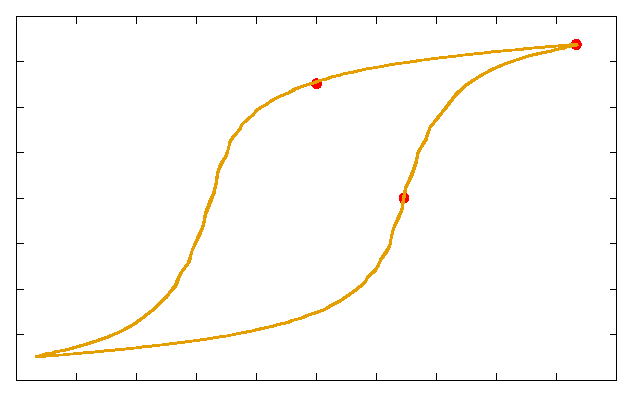
\includegraphics[width={288.00bp},height={180.00bp}]{hystereze}}%
    \gplfronttext
  \end{picture}%
\endgroup

    \captionsetup{type=graph}
    \caption{Měření parametrické závislosti $ x = H(t) $ a $ y = B(t) $ podle vztahů (8) a (6). 
}
\end{figure}

\section{Závěr}

Z měření výchylky kompasu v důsledku magnetu v Gaussových poloháh 1 a 2 jsem změřil horizontální složku intenzity magnetického pole země $ H_z = 16.2  \pm 0.3 \ Am^{-1} $, odkud jsem dopočítal indukce $ B_z = 20.4 \pm 0.3\ \mu T $, která odpovídá tabulková hodnota v Brně je $ Bz = 20.344\ \mu T $. 

Použitím obvodu z obrázku 2 jsem změřil hysterezní křivku některého feromagnetického materiálu a vykreslil ji do grafu 1. Odečtená koercitivní síla byla $ H_C = 29.1\ Am^{-1} $, takže bychom tento materiál řadili mezi magneticky měkké.

\begin{thebibliography}{0}
\bibitem{tabulky} Hustota pevných látek. Dostupné z~\url{http://www.converter.cz/tabulky/hustota-pevne.htmf}.   
\end{thebibliography}

\end{document}
